\documentclass{beamer}

\usepackage[T1,T2A]{fontenc}
\usepackage[utf8]{inputenc}

\usepackage{amsmath}
\usepackage{wrapfig}

\usepackage{bsuslides}

% \graphicspath{ {img/} }

\title{АНАЛИЗ И РАЗРАБОТКА РАСПРЕДЕЛЁННОЙ АРХИТЕКТУРЫ ЭКСПЛУАТАЦИИ НЕЙРОННЫХ СЕТЕЙ\\}
\subtitle{Дипломная работа}
\author{Ларин Егор Сергеевич}
\institute[БГУ]{Белорусский государственный университет \\ ФПМИ, КТС, 4 курс \\ руководитель: старший преподаватель Шолтанюк С. В.}
\date{Минск, 2024}

%\nofiles
\begin{document}

\frame{\titlepage}

\begin{frame}
	\frametitle{Микросервисы}
	\begin{itemize}
		\item В последние годы микросервисная архитектура значительно приобретает популярность в области разработки ПО. 
		\item Использование микросервисной помогает решить вопросы масштабируемости.
	\end{itemize}
	\centering
	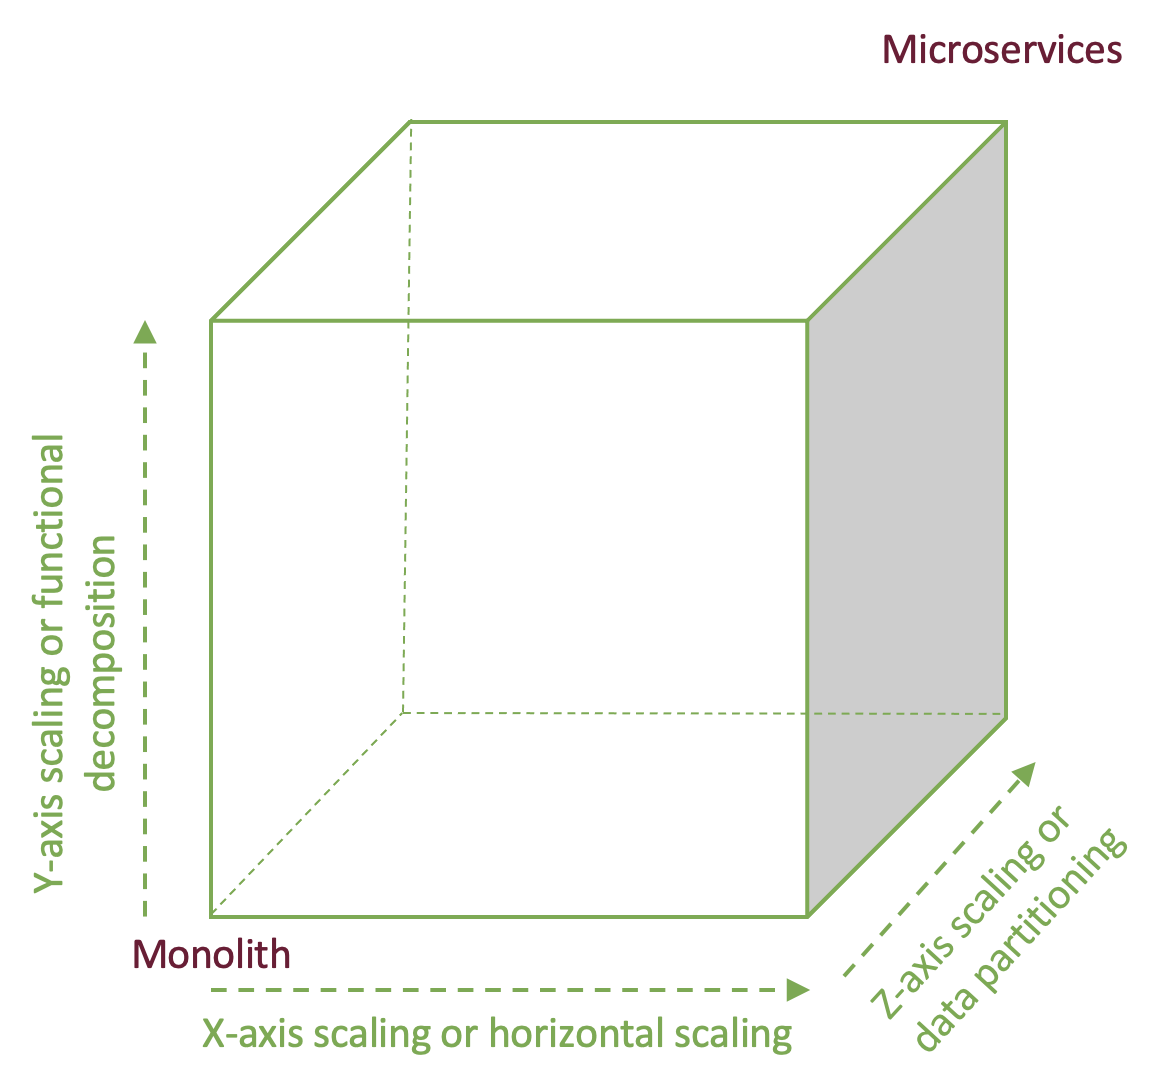
\includegraphics[height=5cm]{img/cube.png}
\end{frame}

\begin{frame}
	\frametitle{Микросервисный монолит}
	\begin{itemize}
		\item Внедрение микросервисов порождает другие проблемы, которые необходимо решать с помощью современных инструментов.
	\end{itemize}
	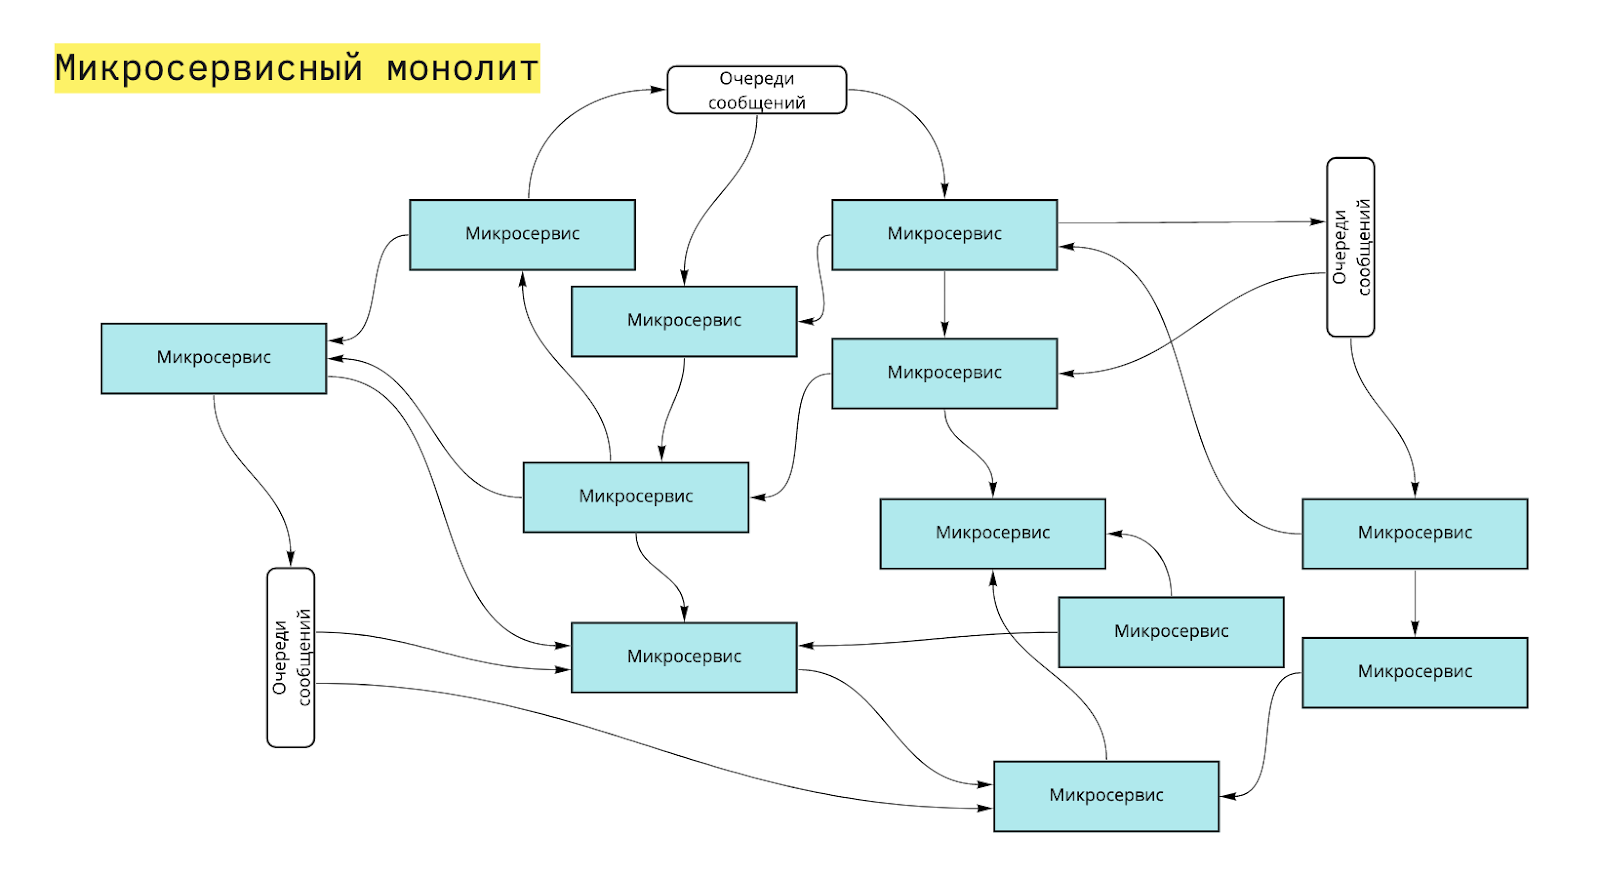
\includegraphics[height=5cm]{img/mon.png}
\end{frame}

\begin{frame}
	\frametitle{Задача сервиса генерации изображений}
	\begin{enumerate}
		\item Обработка входного запроса с параметрами генерации изображения 
		\item Обработка запросов о статусе генерации изображения
		\item Обработка запроса отмены генерации
		\item Обработка запроса получения сгенерированного изображения
	\end{enumerate}
\end{frame}

\begin{frame}
	\frametitle{Общий балансер и проксирование трафика}
	\begin{itemize}
		\item Легче всего в реализации
		\item Плохо масштабируется и предоставляет слабые гарантии обработки сообщений
	\end{itemize}
	\centering
	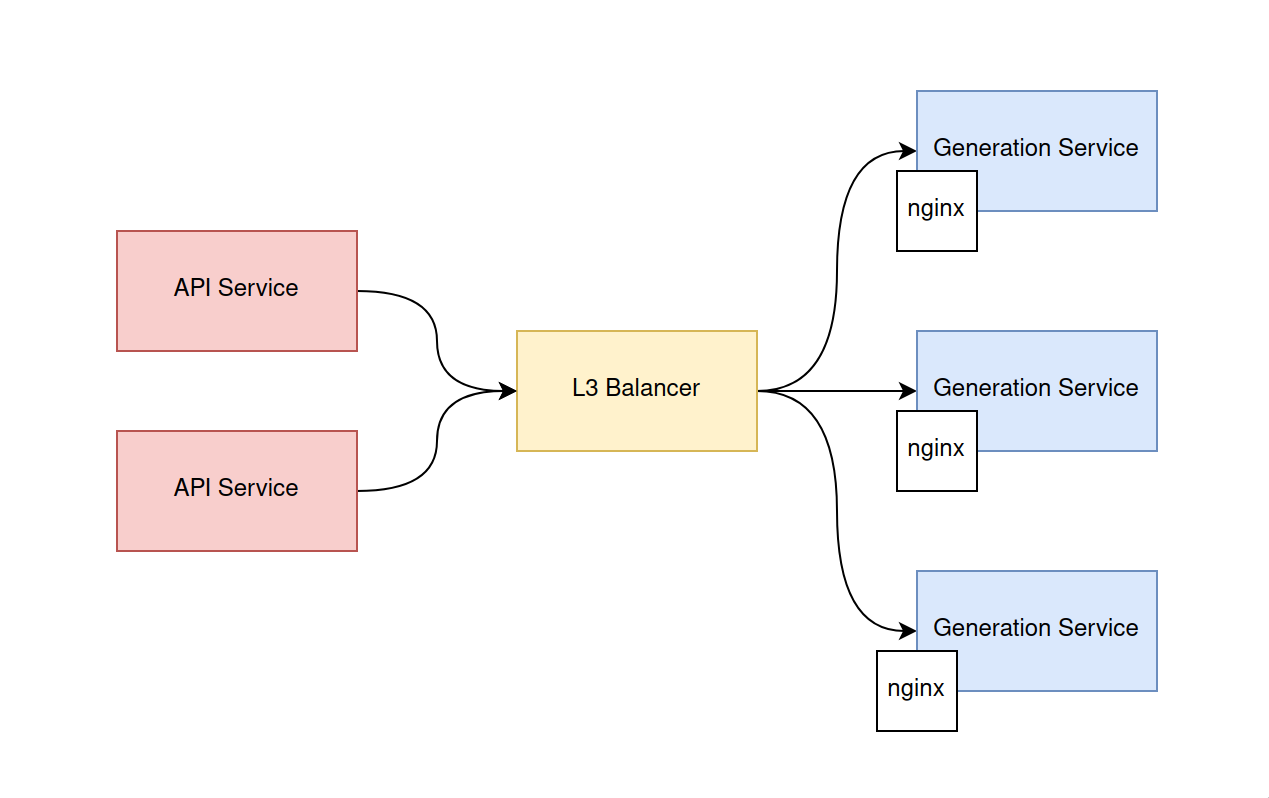
\includegraphics[height=6cm]{img/balancer_old.png}
\end{frame}

\begin{frame}
	\frametitle{Брокер сообщений и асинхронная обработка}
	\begin{itemize}
		\item Устойчива к перегрузкам
		\item Гарантии обработки и порядка
	\end{itemize}
	\centering
	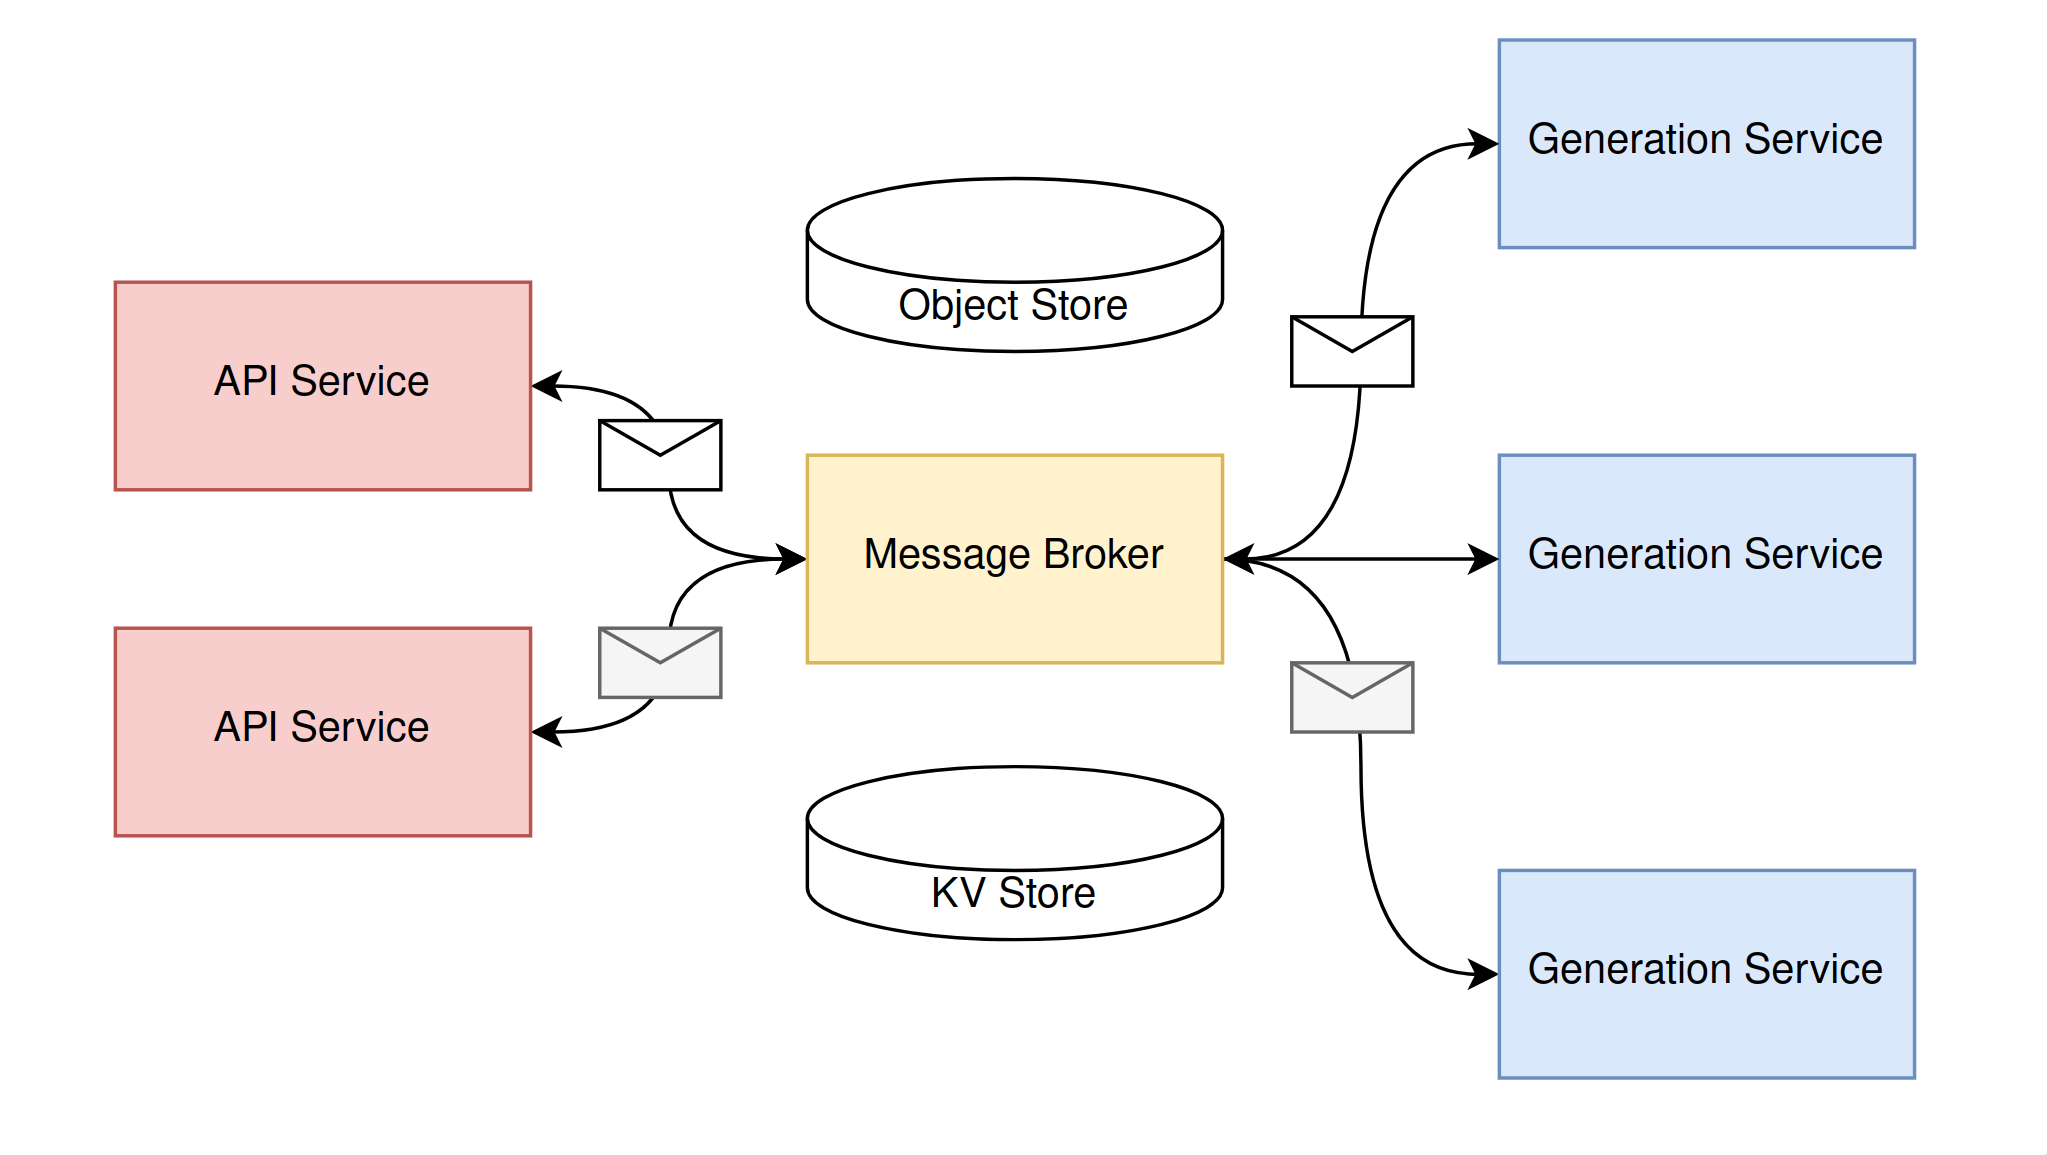
\includegraphics[height=6cm]{img/arch_new.png}
\end{frame}

\begin{frame}
	\begin{itemize}
		\item Минимальные тайминги и высокая надежность
		\item Требует дополнительной разработки для поддержки другой среды исполнения
	\end{itemize}
	\frametitle{Нативная реализация}
	\centering
	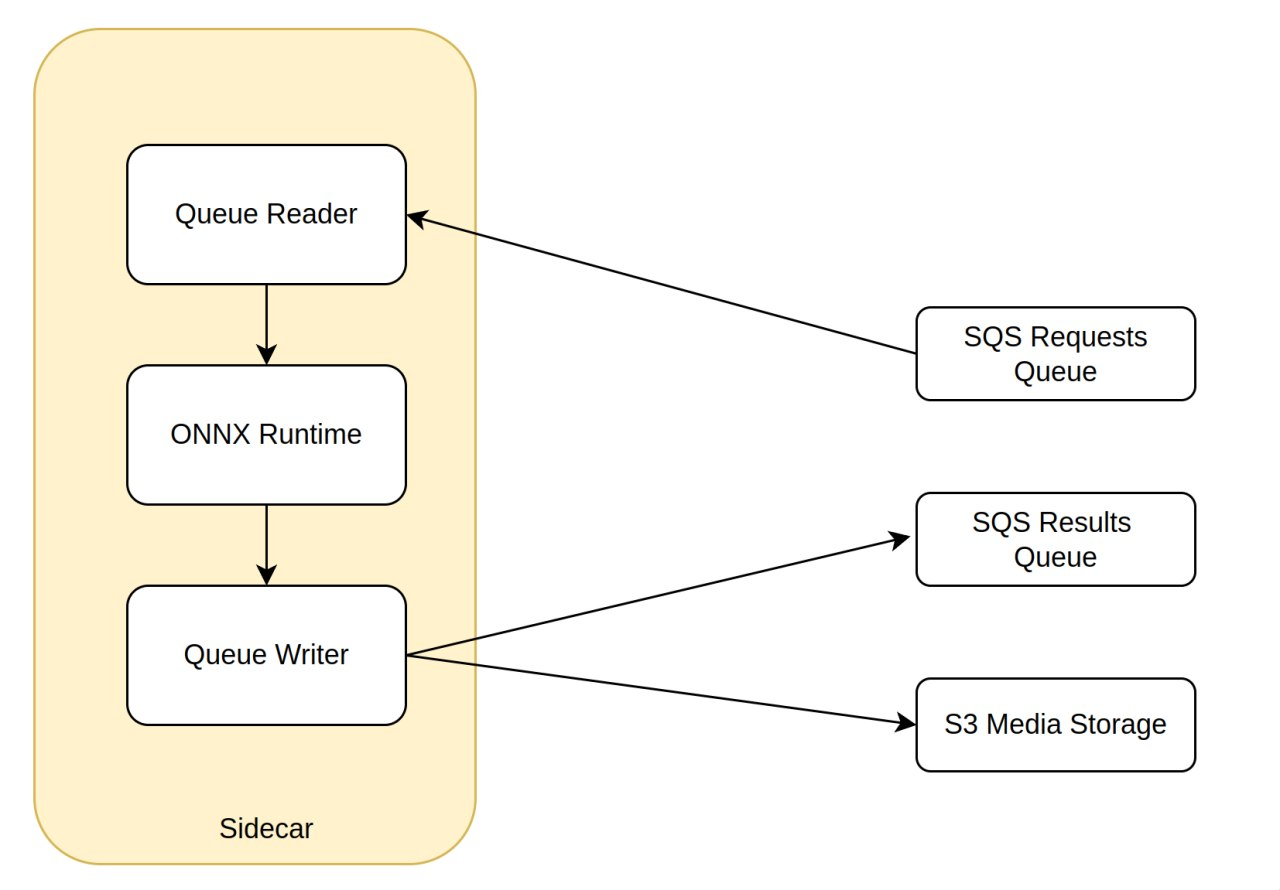
\includegraphics[height=5cm]{img/side1.jpg}
\end{frame}

\begin{frame}
	\begin{itemize}
		\item Самый простой подход в реализации
		\item Издержки на передачу данных по сети и сериализацию
	\end{itemize}
	\frametitle{HTTP сайдкар}
	\centering
	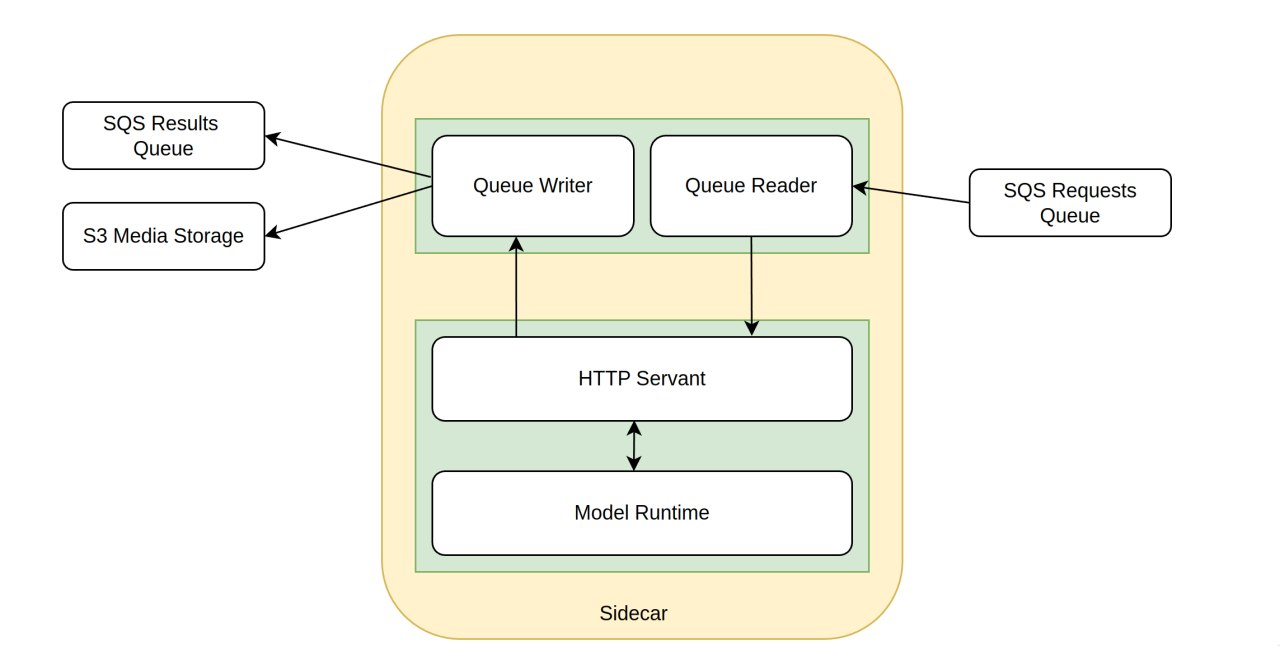
\includegraphics[height=5cm]{img/side2.jpg}
\end{frame}

\begin{frame}
	\begin{itemize}
		\item Более высокая производительность по сравнению с HTTP
		\item Требует разработки и поддержки сетевого протокола
	\end{itemize}
	\frametitle{UDS сайдкар}
	\centering
	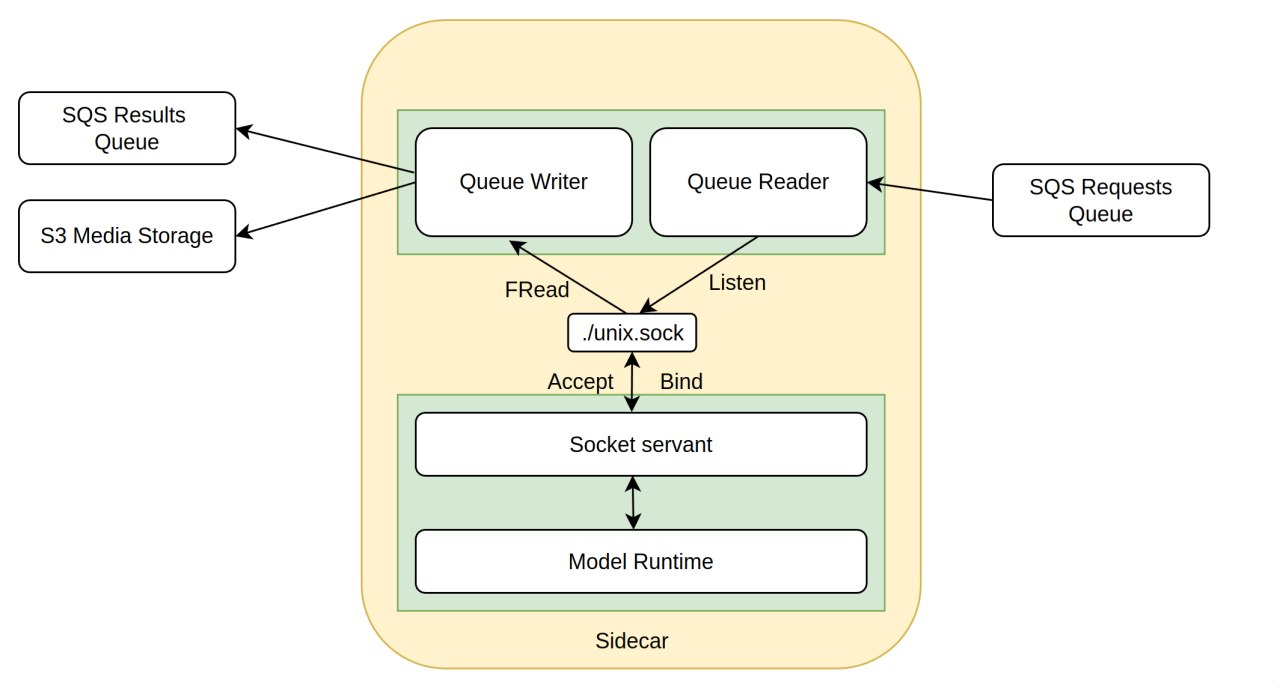
\includegraphics[height=5cm]{img/side3.jpg}
\end{frame}

\begin{frame}
	\begin{itemize}
		\item Отдельный релизный цикл
		\item Инкапсуляция бизнес-логики
	\end{itemize}
	\frametitle{HTTP гейтвей}
	\centering
	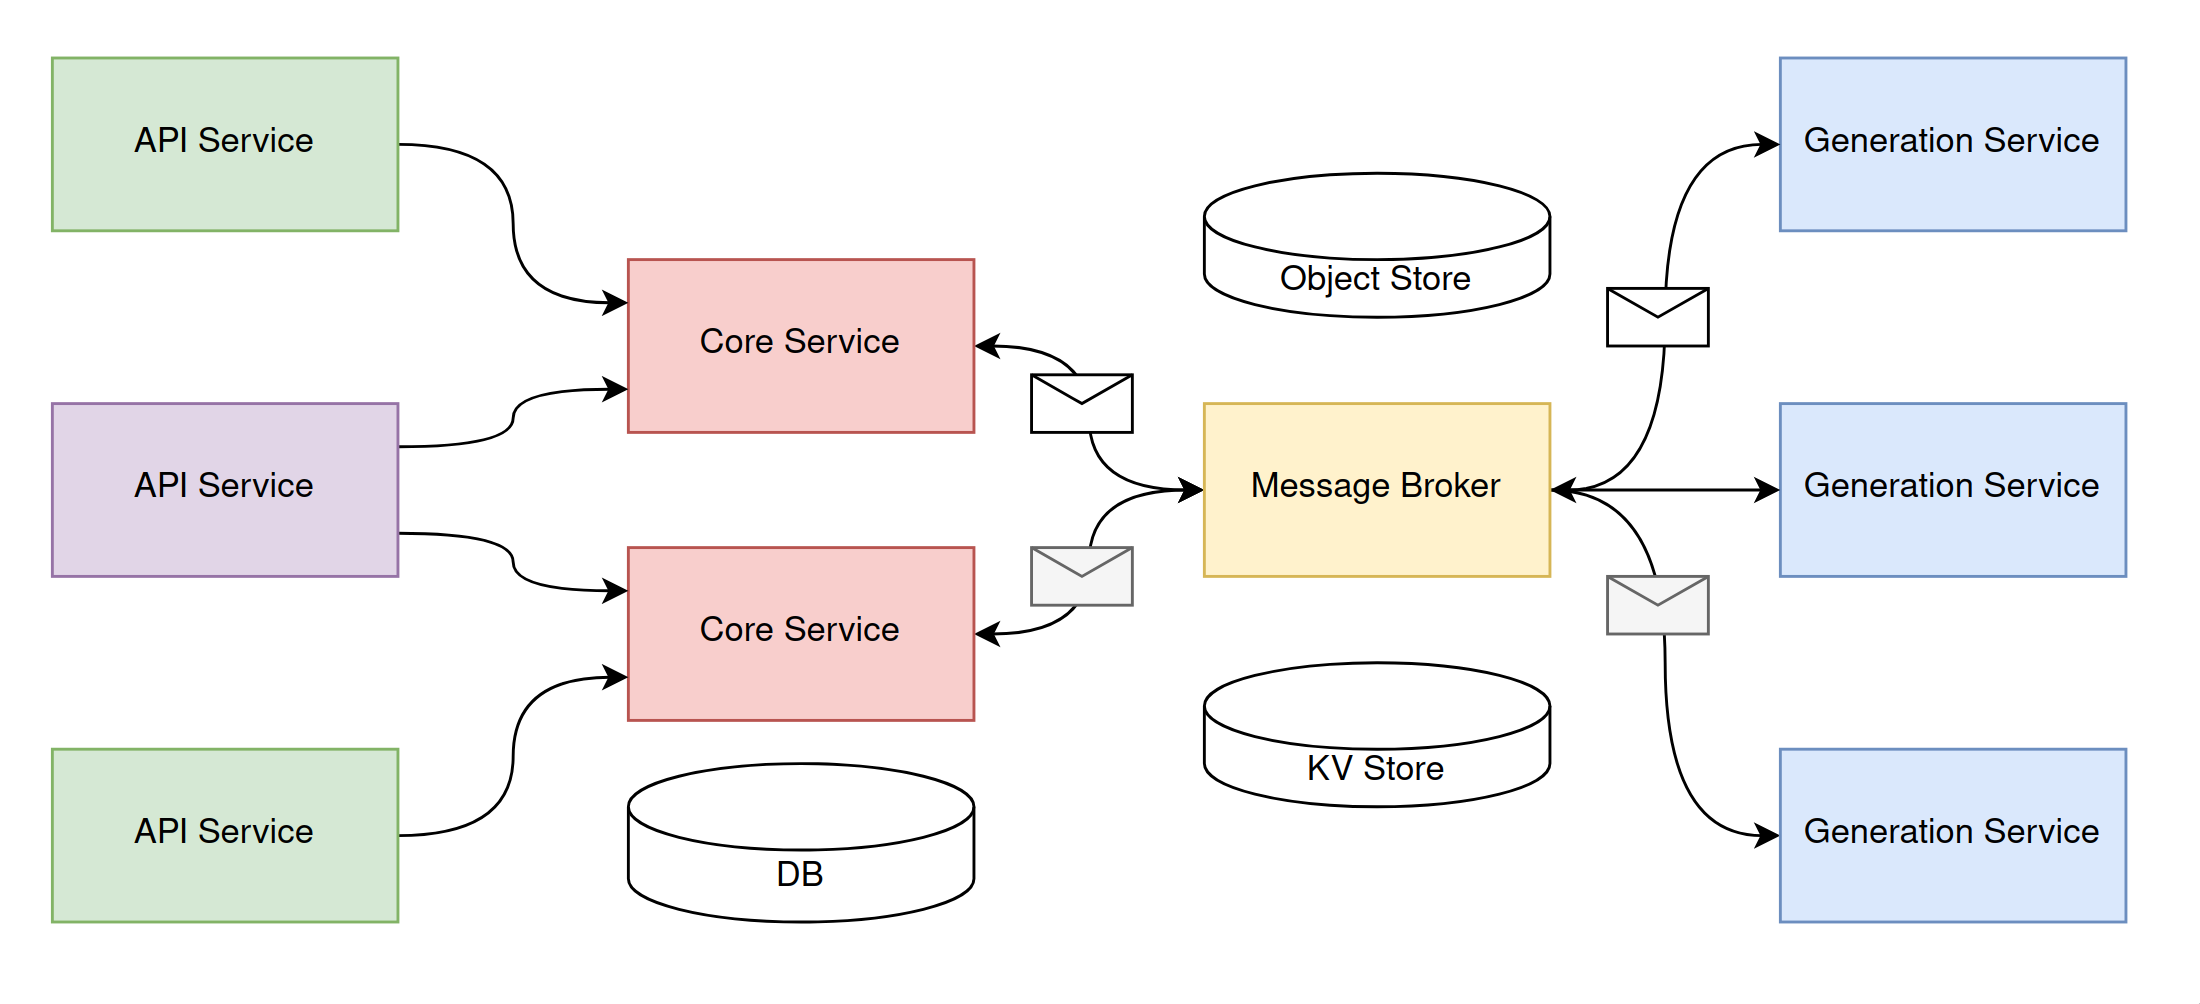
\includegraphics[height=5cm]{img/final.png}
\end{frame}

\begin{frame}
	\frametitle{Заключение}
	\begin{itemize}
	\item В ходе работы было рассмотрено понятие микросервисной архитектуры и произведен обзор имеющихся средств и методологий разработки, применяющихся для коммуникации веб-сервисов.
	\item Результатом работы стала разработка программного обеспечения для генерации изображений с помощью нейронной сети с сетевым интерфейсом. 
	\item Рассмотрены подходы общения разных процессов и проанализированы достоинства и недостатки каждого из методов.
	\end{itemize}
\end{frame}

\begin{frame}
	\frametitle{Источники}
	\begin{enumerate}
		\item Микросервисы: паттерны разработки и рефакторинга / Крис Ричардсон. - Санкт-Петербург [и др.] : Питер, Прогресс книга, 2020. - 542 с. -  (Библиотека программиста). 
		\item Высоконагруженные приложения: программирование, масштабирование, поддержка: [перевод с английского] / Мартин Клеппман. - Санкт-Петербург [и др.] : Питер, Прогресс книга, 2018. - 637 с. -  (Бестселлеры O'Reilly). 
		\item Marek Bolanowski, Kamil Zak, Andrzej Paszkiewicz, Maria Ganzha, Marcin Paprzycki, Piotr Sowinski, Ignacio Lacalle, and Carlos E. Palau. Eficiency of REST and gRPC Realizing Communication Tasks in Microservice-Based Ecosystems. IOS Press, September 2022..
	\end{enumerate}
\end{frame}

\begin{frame}
	\frametitle{Справочная информация}
	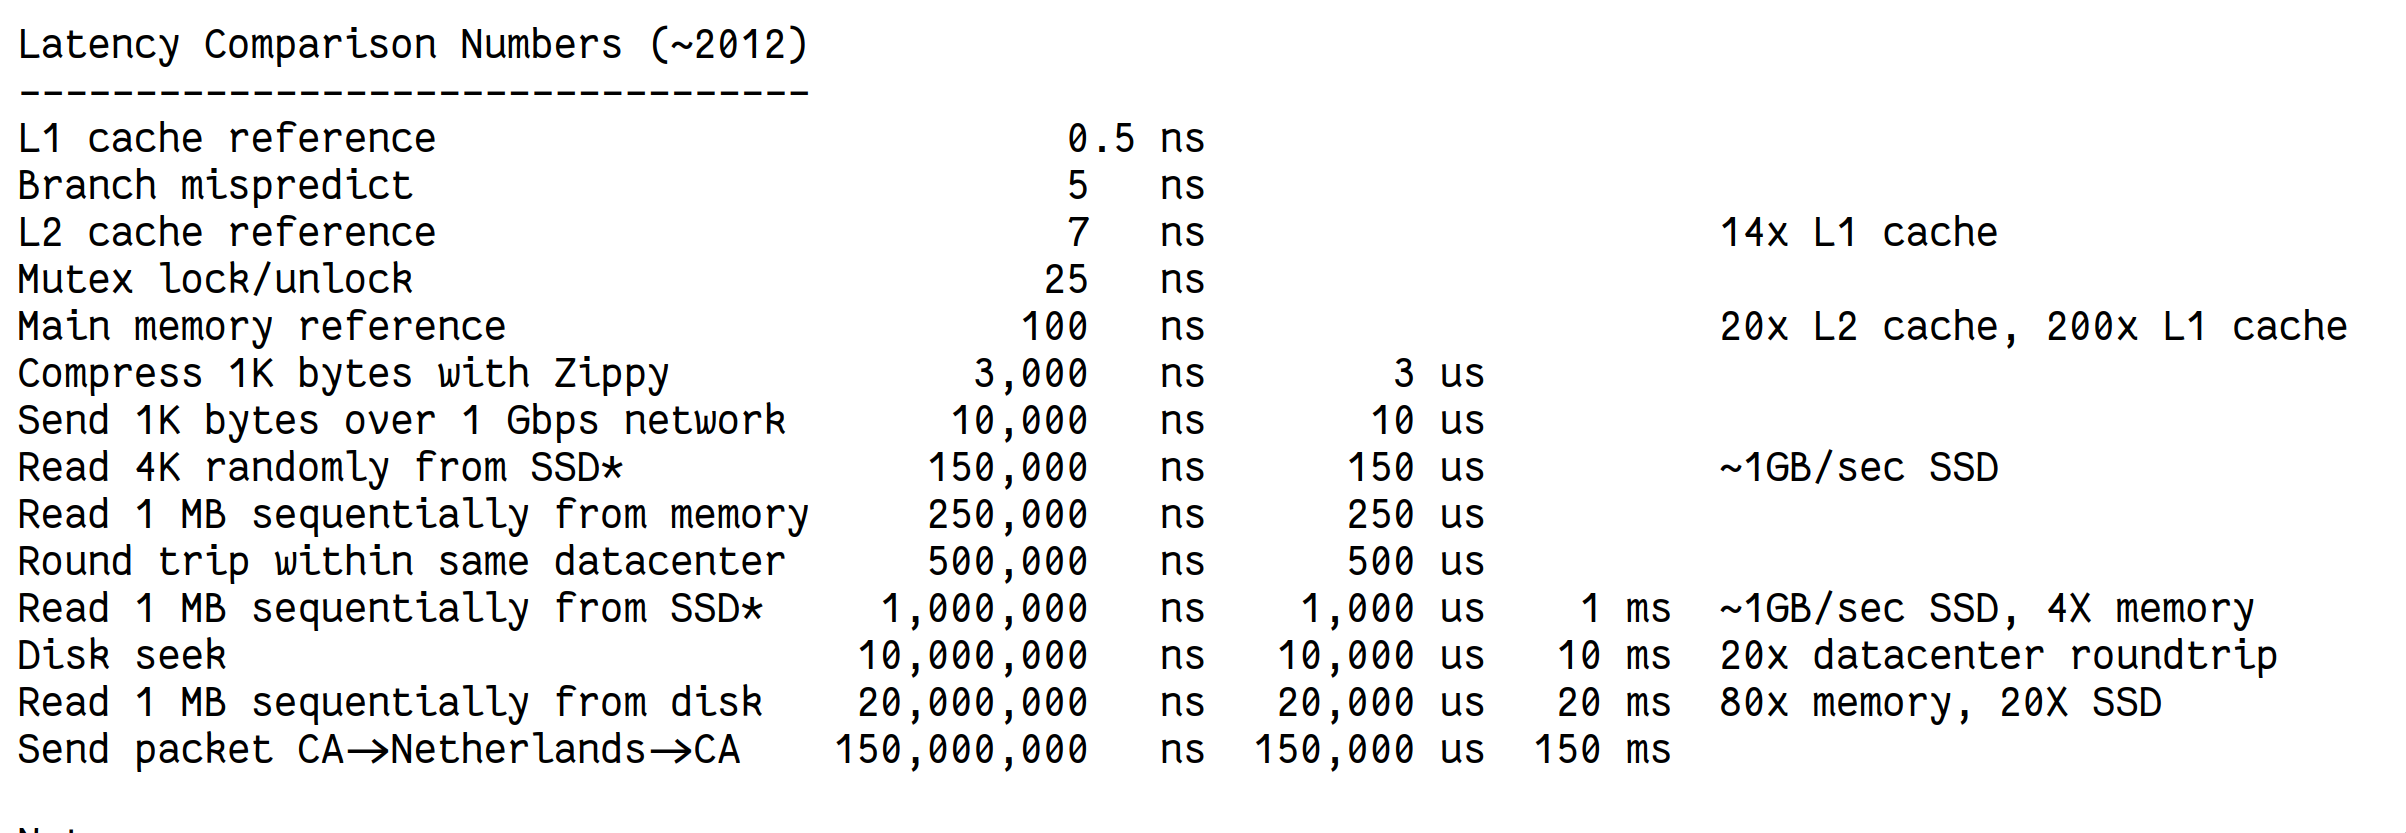
\includegraphics[height=4cm]{img/latency.png}
\end{frame}

\end{document} 
